\subsection*{Pasos}
Los pasos que seguimos se enumerarán enseguida, estos van en orden a los objetivos.
\begin{enumerate}[1.]
    \item{\bfseries Creación de un repositorio:} Primero lo que hicimos fue crear un repositorio en la página de Git-Hub, para suerte ya contabamos con una, despues creamos un proyecto nuevo junto con una rama, cada uno siguió una rama durante el resto del proyecto.
    \item{\bfseries Creación del Documento en Overleaf:} Arnold por su parte creó una cuenta en Overleaf, yo por mi parte ya tenía una, después pocedimos a crear un docuemento.
    \item{\bfseries Descarga de Documentos:} En este paso descargamos los documentos con la ayuda del ya mencionado Batch link Downloader y lo guardamos en una carpeta llamada data.
    \item{\bfseries Orange:} En este paso fue en el que estuvimos más tiempo entretenidos, primero creamos un archivo nuevo y con la ayuda de multifile cargamos todos los archivos que habíamos descargado, una vez cargados procedimos a resolver cada uno de los obhetivos, que veremos enseguida:

        \begin{enumerate}[Obj{e}t{i}vo 1.]
            \item Para el objetivo uno que es: {\bfseries Ordenar las entidades federativas según el crecimiento promedio para cada año durante el periodo que se estudia para la especie “Bovina”} , tuvimos un problema que era que al parecer algunos de los archivos tenían diferentes datos, lo cual ya se nos había recomendado dividir en dos grupos, pero después nos enontramos con otro problema con que algunos de los datos de Asacrificados estaban divididos, por lo cual Orange lo tomaba como datos perdidos, por lo cual seleccionando filas y columnas terminamos por concatenar ambas columnas en una sola; sin embargo nos surgió otro problema el cual era que algunos de los nombres no estaban bien escritos (debido a los acentos) entonces utilizando la búsqueda de Orange encontramos los años en los cuales estaban mal escritos y los corregimos, después de estos procedimientos por fin teniamos un data table sin datos perdidos, por lo cual pasamos a descargar el add-ons Spectroscopy, para obtener los promedios de nuestra tabla. \\
Antes de obtener los promedios filtramos por especie.\\
Se adjuntan las imágenes de lo mencionado anteriormente, en la figura 1 podemos observar el proceso en {\bfseries Orange } de la concatenación y filtrado para obtener todos los datos correspondientes mientras que en la figura. 

            \begin{figure}
            \centering
            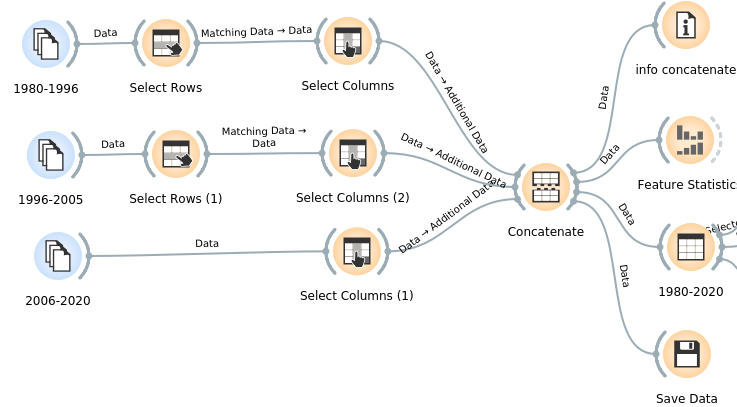
\includegraphics[scale = 0.5]{imagenes/orange1.png}
            \caption{Concatenación de archivos}
            \label{concatenacion}
            \end{figure}
            \begin{figure}
                \centering
                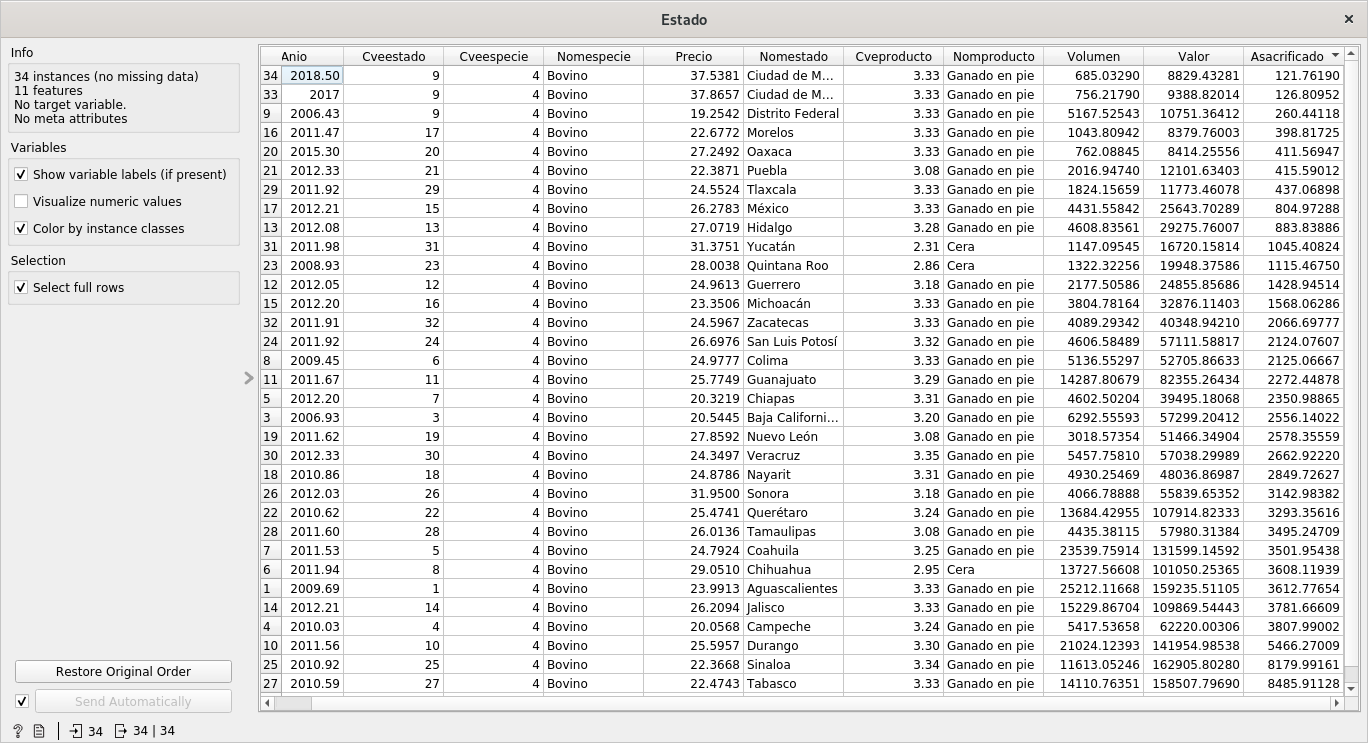
\includegraphics[scale = 0.3]{imagenes/estadosporasacrificado.png}
                \caption{Estados Federativos ordenados por Sacrificados}
                \label{tablesacrificados}
            \end{figure}
            \begin{figure}
                \centering
                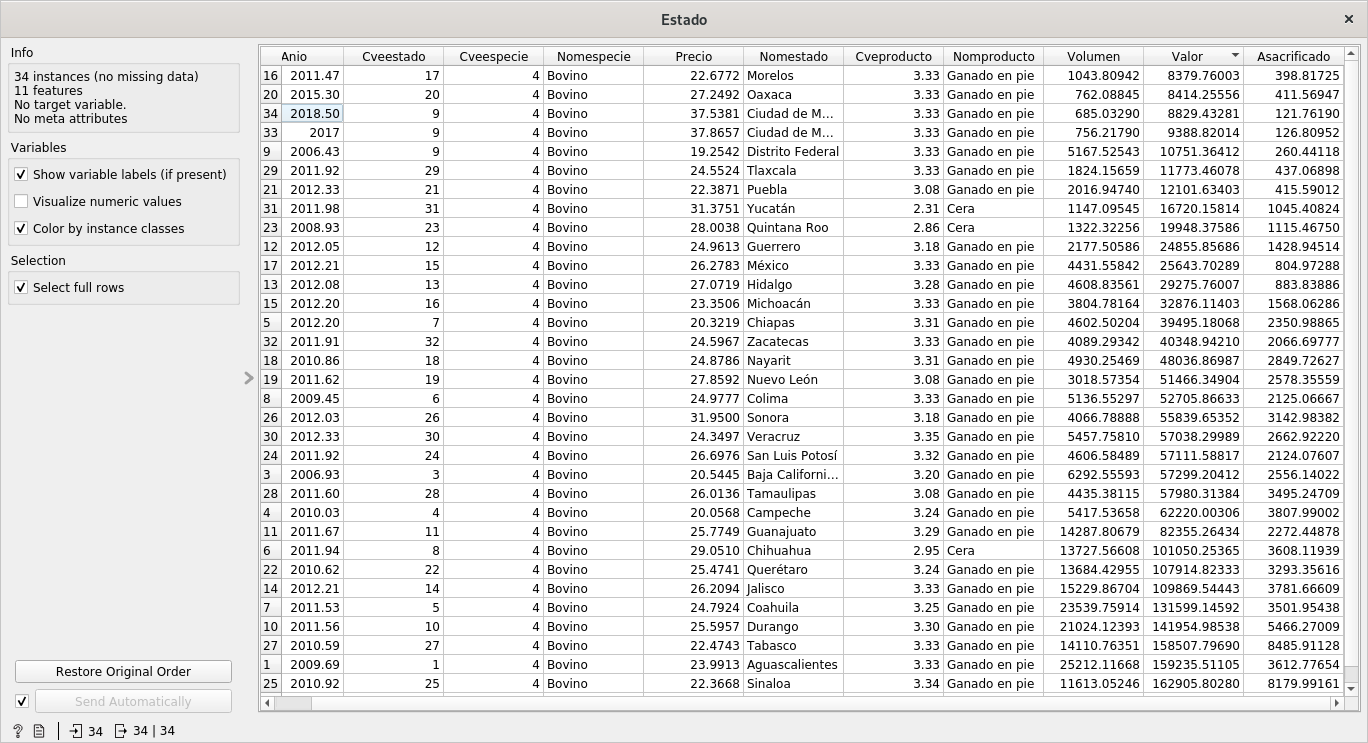
\includegraphics[scale = 0.3]{imagenes/estadosporvalor.png}
                \caption{Estados Federativos ordenados por valor}
                \label{tablevalor}
            \end{figure}
            \newpage
            \item Para el objetivo 2 que es: {\bfseries Ordenar las entidades federativas según el valor promedio de su producción pecuaria para cada año el periodo que se estudia para la especie “Bovina”}, hicimos el mismo procedimiento que el anterior, obteniendo claro la siguiente imagen en la figura 3.
            \item En el objetivo 3: \\ {\bfseries Grafique la relación entre los valores para el crecimiento promedio y el valor promedio establecidos en las tareas anteriores para cada una las entidades: Veracruz, Sonora, Tamaulipas, Sinaloa, Oaxaca. ¿Qué observa?}, primero tuvimos que filtrar los estados por medio de {\bfseries Orange} para solo seleccionar los estados que nos pedían. \\
Una vez que tenemos el filtro procedimos a obtener la siguiente gráfica en la cual se ve que: Sinaloa fue el estado con un promedio más alto tanto en producción como en valor, enseguida se adjuntan las imágenes de lo obtenido.\\
Se observa que Sinaloa es el mayor en ambas gráficas.
            \begin{figure}[htb!]
                \begin{minipage}[b]{0.5\linewidth} %Una minipágina que cubre la mitad de la página
                \centering
                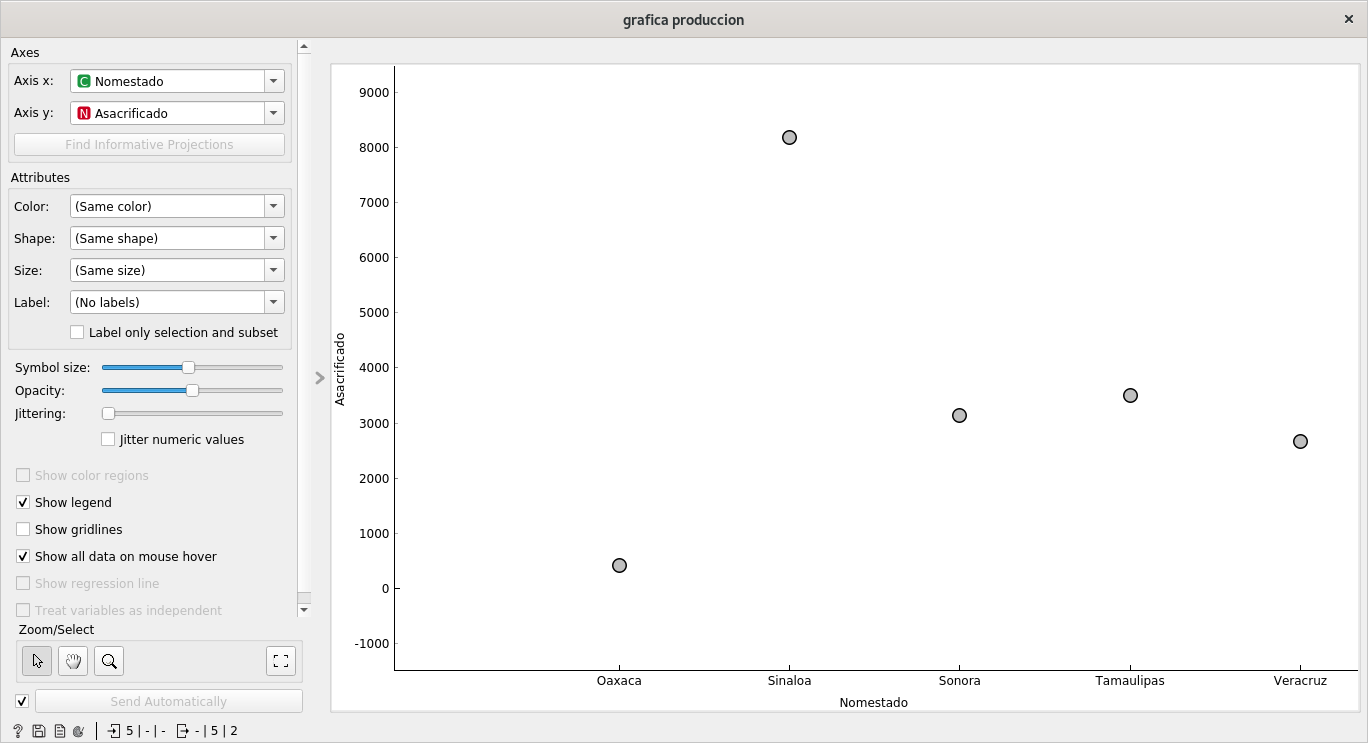
\includegraphics[width = 8cm]{imagenes/graficaestados-sacrificados.png}
                \caption{Gráfica Estados ordenados por sacrificio}
                \label{graficaestadossacrificio}
                \end{minipage}
                \hspace{0.5cm} % Si queremos tener un poco de espacio entre las dos figuras
            \begin{minipage}[b]{0.5\linewidth}
                \centering
                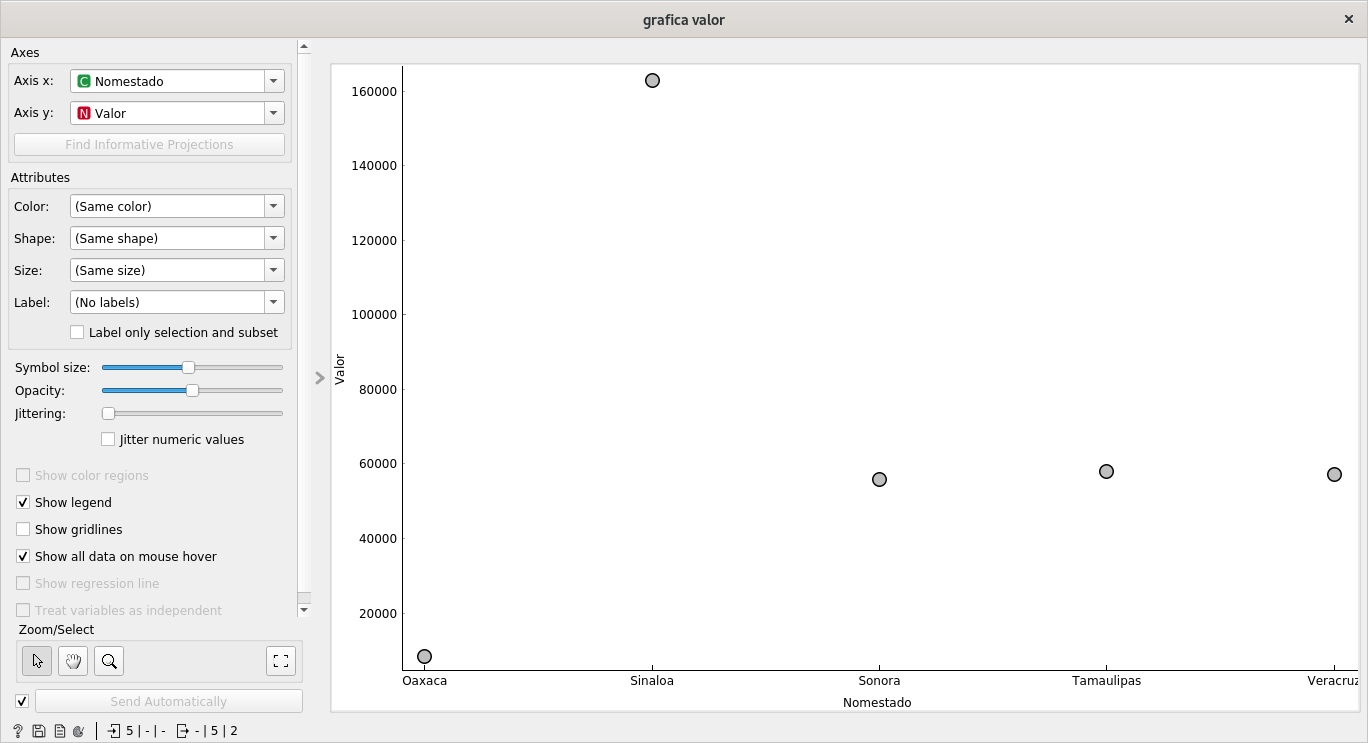
\includegraphics[width = 8 cm ]{imagenes/graficaestados-valor.png}
                \caption{Gráfica Estados ordenados por valor}
                \label{graficaestadosvalor}
                \end{minipage}
            \end{figure}
\newpage
            \newpage
            \item En este objetivo es en el que decidiremos nuestra hipótesis, la cual si recordamos era que no existía ninguna correlación entres los valores de nuestros registros.\\
Una vez que teniamos nuetra tabla filtrada por los datos pedidos en el objetivo anterior pasamos a obtener su coeficientes de correlación de Spearman, los cuales se muestran en la siguiente imagen \\
            \begin{figure}[h]
                \centering
                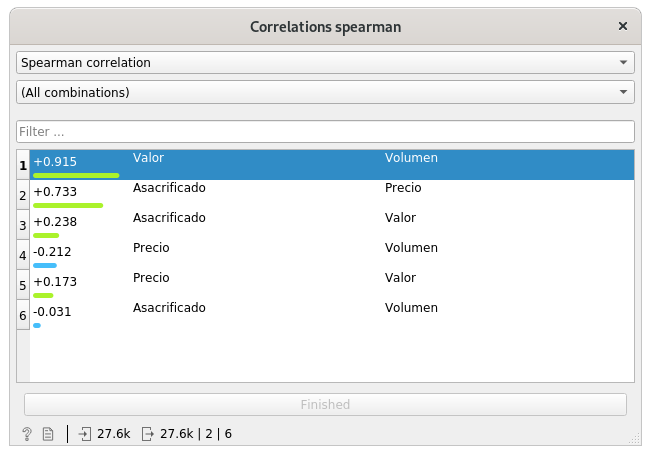
\includegraphics[scale = 0.3]{imagenes/correlacion.png}
                \caption{Correlación de Spearman}
                \label{correlacion}
            \end{figure}
\\Como podemos ver existen varias correlaciones, pero las más importantes son las existentes entre Valor-Volumen y Asacrificado-Precio, por lo cual podemos rechazar nuestra hipótesis.
            
            \item Para este objetivo tuvimos que filtrar de nuevo como se ve en la figura \ref{filtrosnuevos}, ya que solo nos pedían los estados de Veracruz y Tamaulipas y además teniamos que dividir el año 2020; después de esto pasamos a crear un guardado e incorporarlo en el documento, para hacer una predicción como se muestra en la figura \ref{tercerfiltro}, de igual manera cargamos los datos reales y los graficamos enseguida se adjuntan ambas imágenes.
\begin{figure}[h]
    \centering
    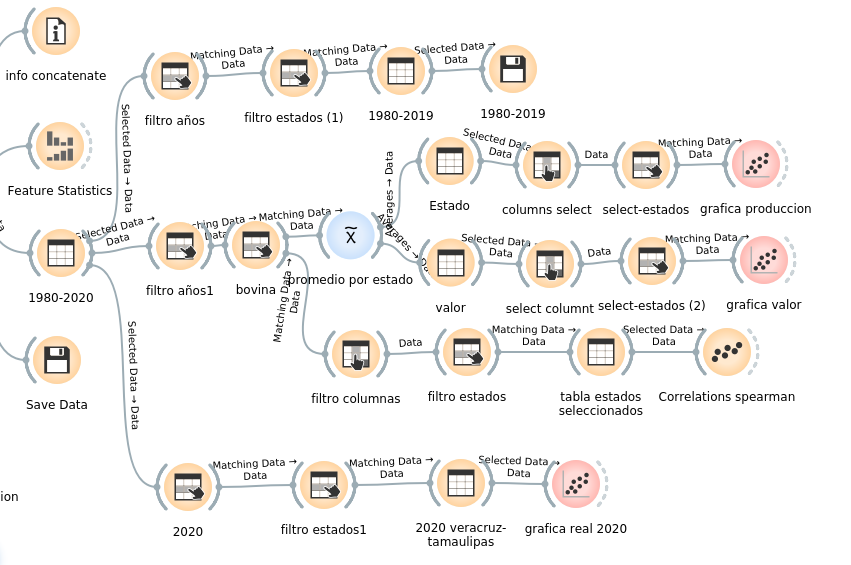
\includegraphics[scale = 0.4]{imagenes/Orange2.png}
    \caption{Filtros Nuevos}
    \label{filtrosnuevos}
\end{figure}
\begin{figure}[h]
    \centering
    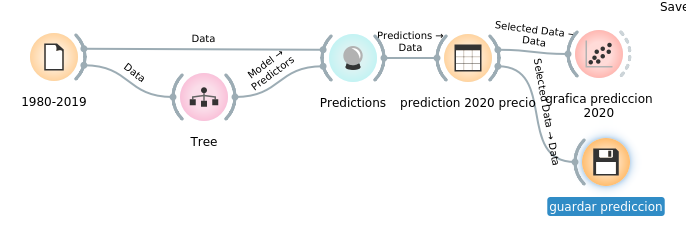
\includegraphics[scale = 0.5]{imagenes/orange3.png}
    \caption{Tercer filtro}
    \label{tercerfiltro}
\end{figure}
\begin{figure}[htb!]
\begin{minipage}[b]{0.5\linewidth} %Una minipágina que cubre la mitad de la página
\centering
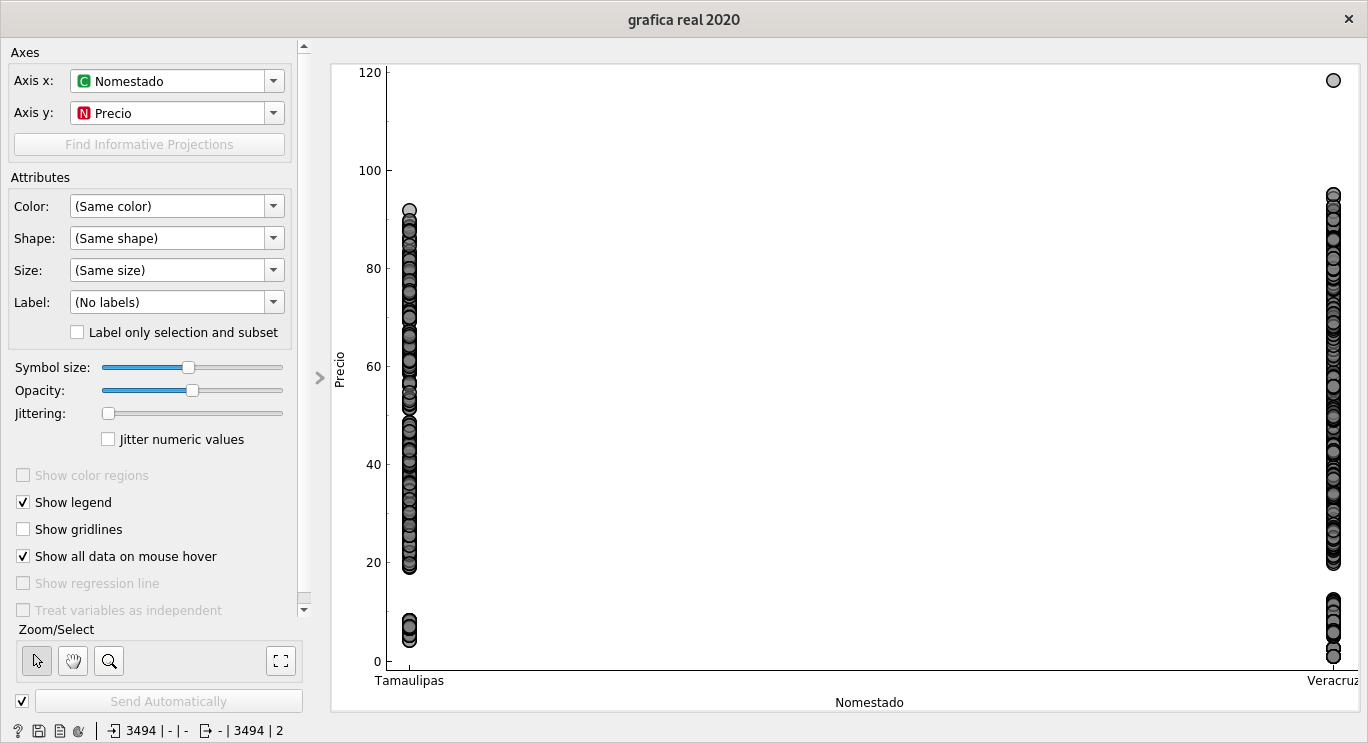
\includegraphics[width=8cm]{imagenes/grafica-real-2020.png}
    \caption{Gráfica real 2020}
    \label{graficareal}
\end{minipage}
\hspace{0.5cm} % Si queremos tener un poco de espacio entre las dos figuras
\begin{minipage}[b]{0.5\linewidth}
\centering
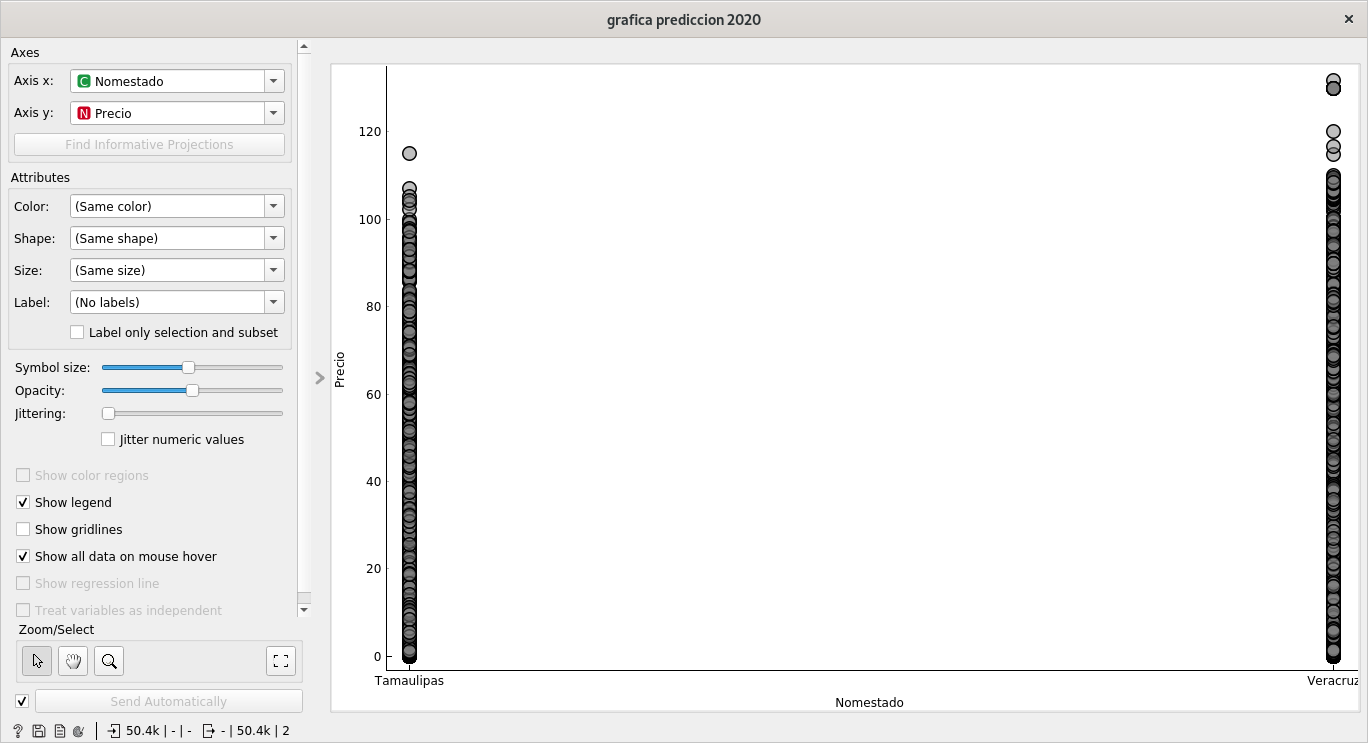
\includegraphics[width=8cm]{imagenes/grafica-prediccion.png}
    \caption{Gráfica predicción 2020}
    \label{graficaprediccion}
\end{minipage}
\end{figure}
\newpage
Como podemos ver la gráfica entre ambas es demasiado similar.
Entonces de cierto modo podemos decir que nuestra predicción es demasiado cerca a los datos reales.
        \end{enumerate}


\end{enumerate}